\documentclass{article} % For LaTeX2e
\usepackage{overall_style,times, natbib}

\usepackage{graphicx}
\usepackage{hyperref}
\usepackage{url}
\usepackage{subfigure}
\usepackage{amsmath}
\usepackage{amssymb}
\usepackage{mathrsfs}
\usepackage{float}
\usepackage{caption}

\title{Introduction to Deep Learning - Assignment 0}

\author{Niels de Klerk (s3640477), Vincent Franken (s3682633), Phoebe Dos Santos Cordeiro (s3555380)}

\iclrfinalcopy

\begin{document}

\maketitle
\section{Introduction}

\section{Task 1}
\subsection{Task 1.1: Means and distances of digits}
The first step is to calculate the means for each respective digit vector. To this end, for each digit, we make use of a mask based on the training output to then average over the respective inputs. By using these averages of the input vectors, we calculate the distance between the means of each digit vector.

\begin{figure}[h]
    \centering
    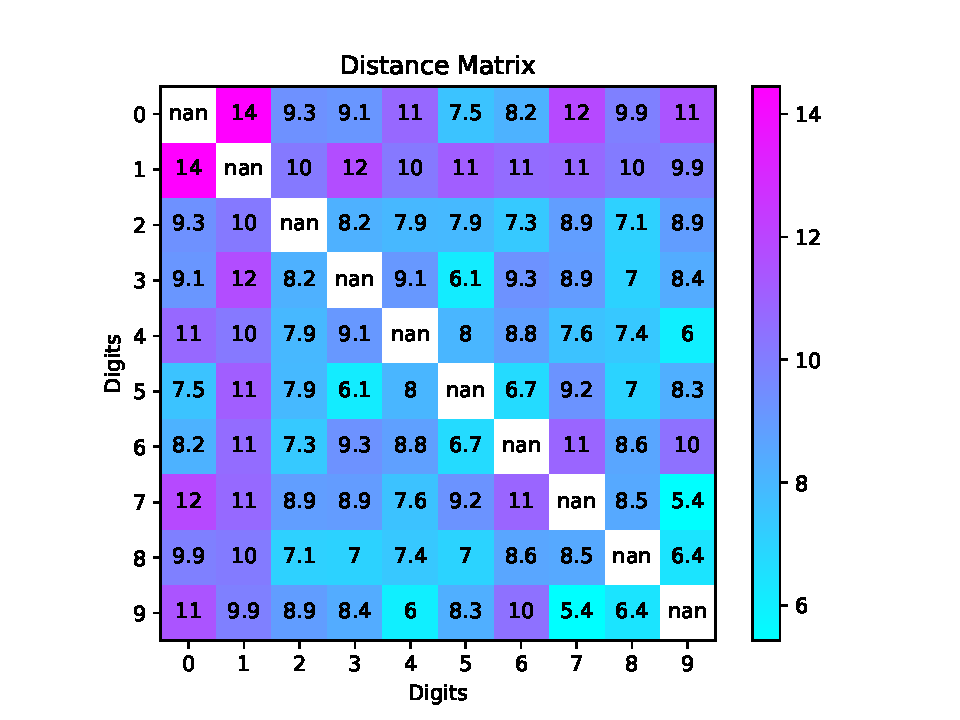
\includegraphics[width=0.4\linewidth]{imgs/dist_matrix.pdf}
    \caption{Distance matrix between digit vector means}
    \label{fig:dist_mat}
\end{figure}
\label{sec:dimred}
\subsection{Task 1.2: Dimensionality reduction}
While PCA doesn't give us a very clear picture of the distances between the digits, t-SNE and UMAP show us the same trends. Even though the placement of the points might be different between the plots their neighbours remain similar. For both plots we can see that 0 and 1 are at opposite ends while 9 and 7 are either very close or merging, which agrees with our conclusions from before.
\begin{figure}[h]
    \centering
    \subfigure[]{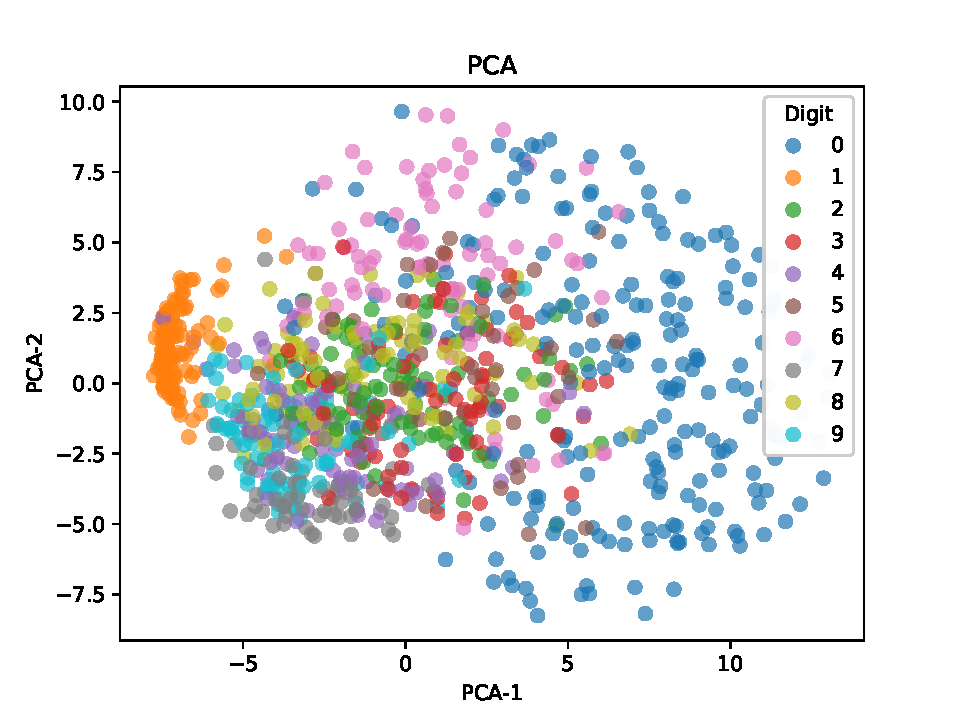
\includegraphics[width=0.3\textwidth]{imgs/PCA.pdf}}
    \subfigure[]{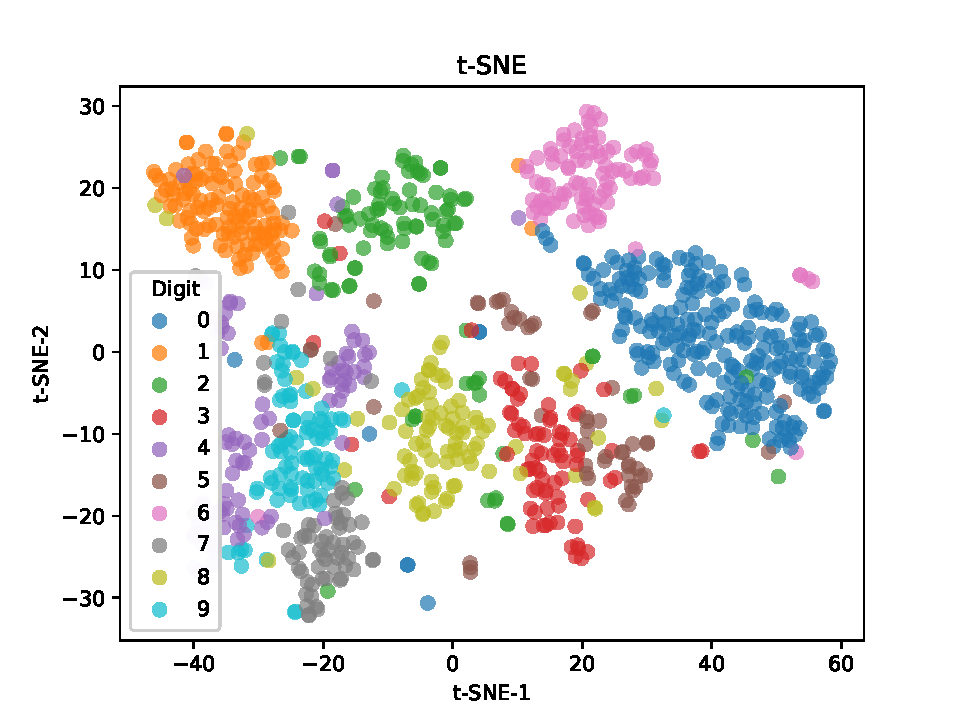
\includegraphics[width=0.3\textwidth]{imgs/tSNE.pdf}}
    \subfigure[]{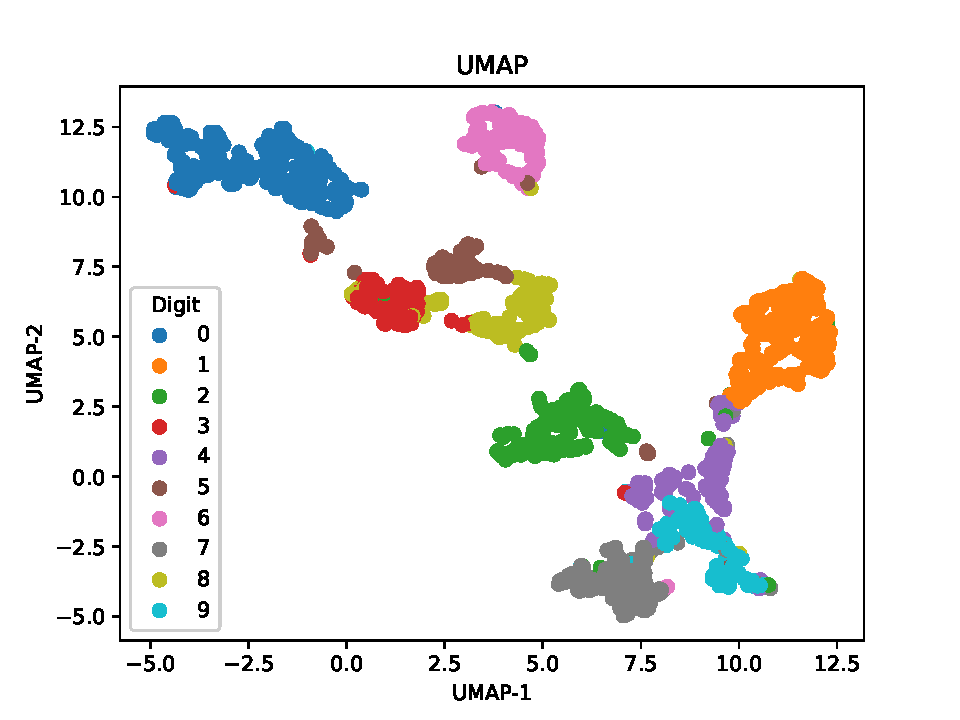
\includegraphics[width=0.3\textwidth]{imgs/umap.pdf}}
    \caption{Dimensionality reduction algorithms: (a) PCA (b) t-SNE (c) UMAP}
    \label{fig:dimred}
\end{figure}
\subsection{Task 1.3: Nearest Neighbour}
By taking all our image vectors and calculating their distances to our previously obtained digit mean vectors, we classify each image with the digit it's closest to. This gives us an accuracy of 86.35\% on the training set and 80.4\% on the test set. 
\begin{figure}[h]
    \centering
    \subfigure[]{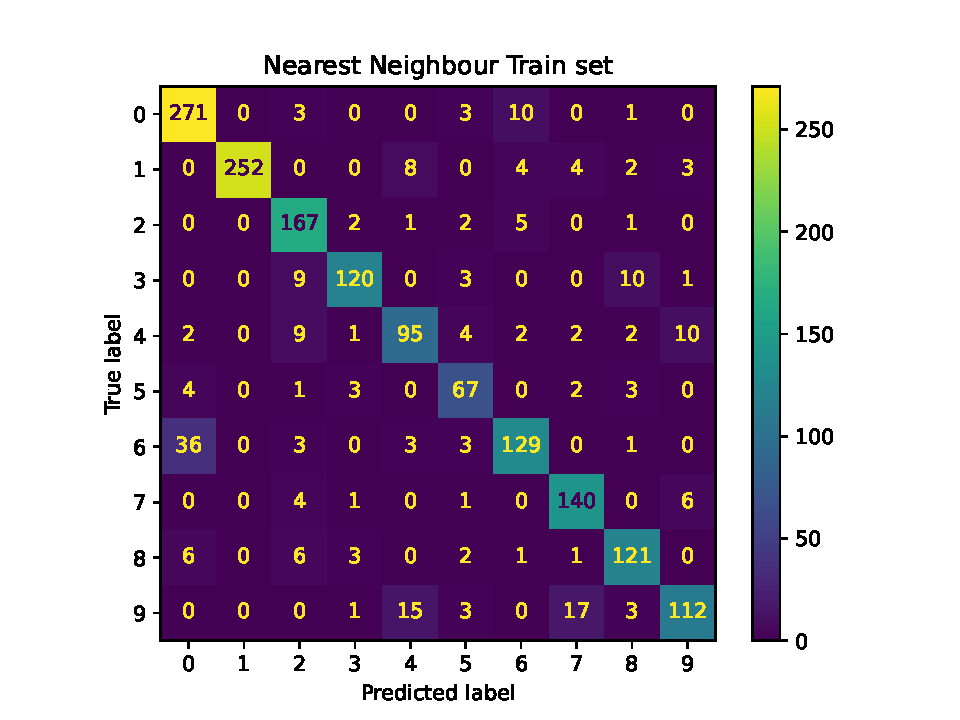
\includegraphics[width=0.4\textwidth]{imgs/NN_train.pdf}}
    \subfigure[]{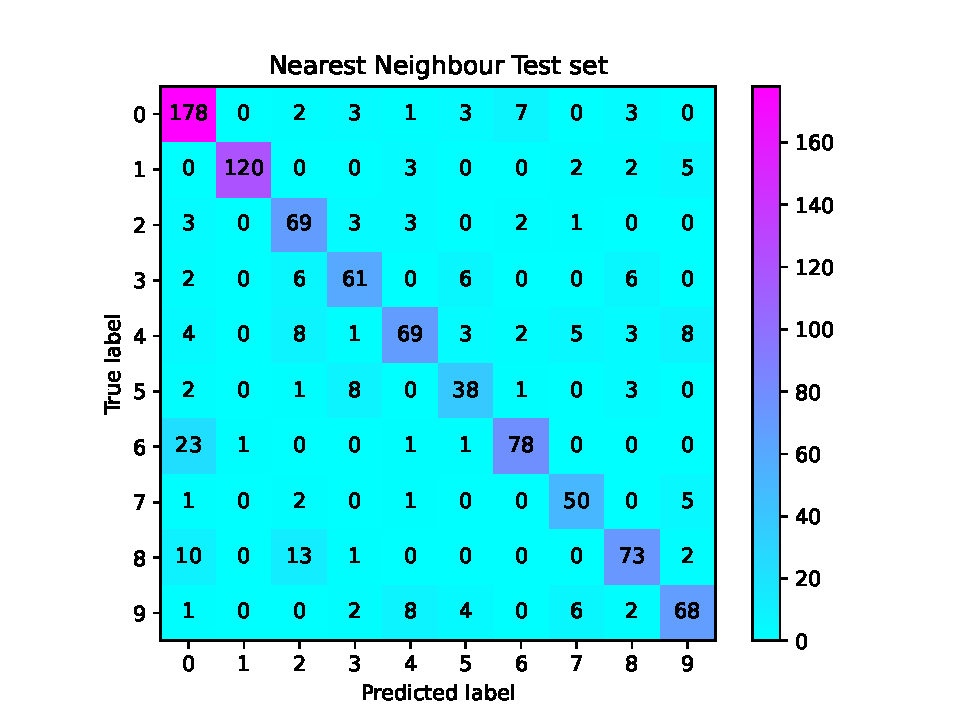
\includegraphics[width=0.4\textwidth]{imgs/NN_test.pdf}}
    \caption{Nearest Neighbour classifier confusion matrix (a) training set (b) test set}
    \label{fig:NN}
\end{figure}
\subsection{Task 1.4: K Nearest Neighbour}
For this task we make use of the scikit-learn package with its KNN classifier class. We use n\_neighbours = 3 for our parameters and then fit the classifier to our training data. \\
\begin{figure}[h]
    \centering
    \subfigure[]{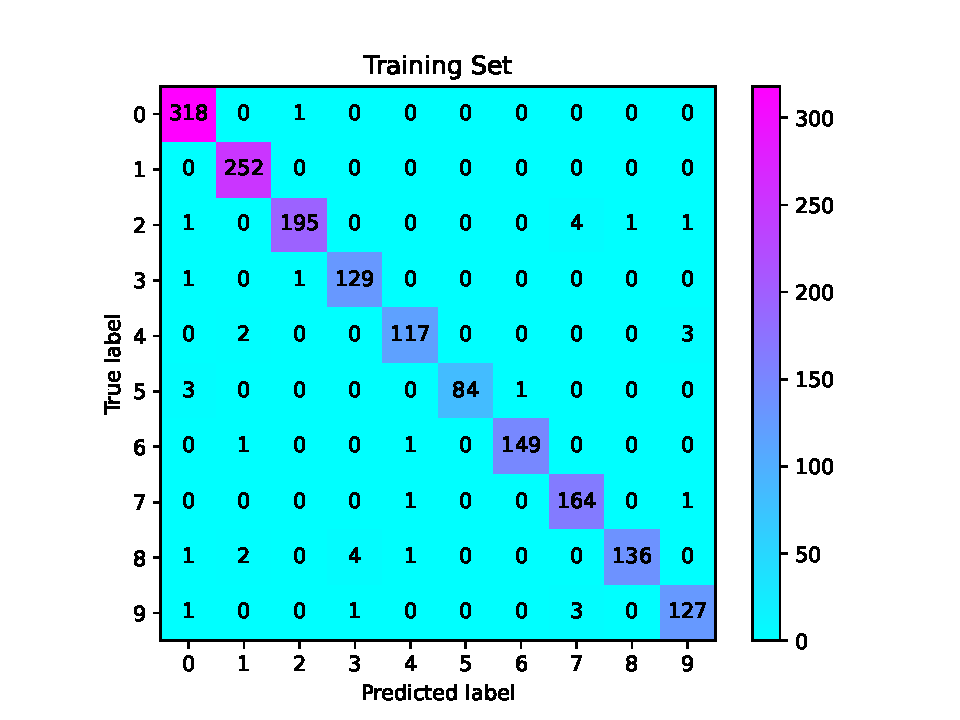
\includegraphics[width=0.4\textwidth]{imgs/KNN_train.pdf}}
    \subfigure[]{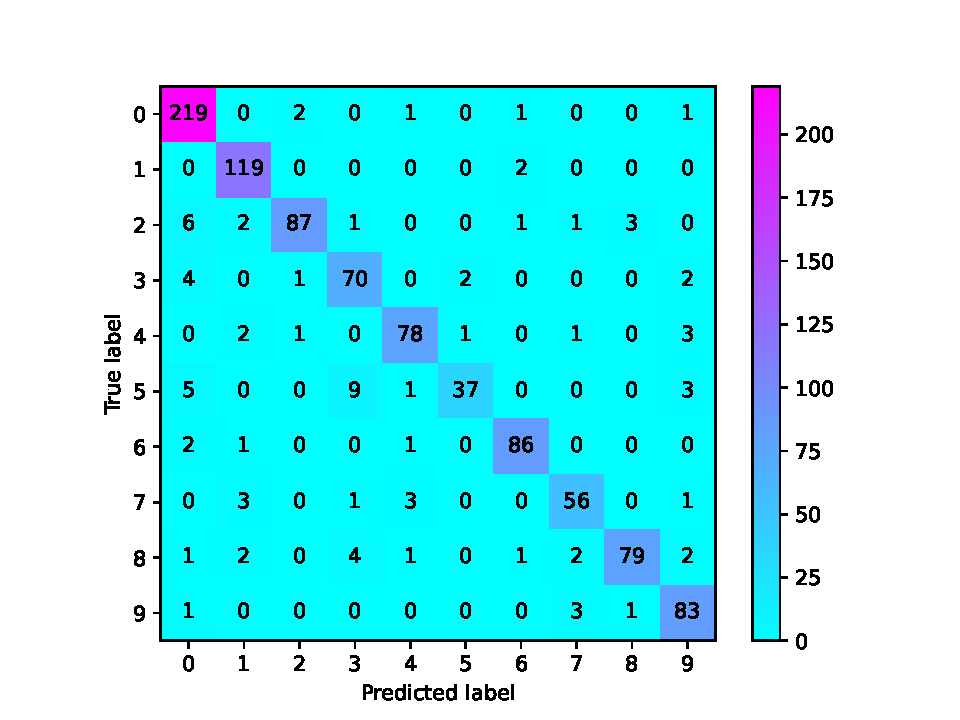
\includegraphics[width=0.4\textwidth]{imgs/KNN_test.pdf}}
    \caption{Nearest Neighbour classifier confusion matrix (a) training set (b) test set}
    \label{fig:KNN}
\end{figure}\\
By looking at the four confusion matrices from Figure \ref{fig:NN} and Figure \ref{fig:KNN} we notice first that KNN is better at classifying than the naive NN method. A second trend we can observe is that while KNN struggles most at distinguishing 3 from 5, the NN method doesn't and instead struggles a lot more with 0 and 6. Neither of these struggles are what we expected from our previous look into the data in \ref{sec:dimred}. Looking at our UMAP (Figure \ref{fig:dimred}) results, these struggles make sense as some digits may fall in between the two digits in terms of distance, which then leads them to being classified wrongly.

Training set accuracy: 97.9\% Test set accuracy: 91.4\%

\section{Task 2: Multi-class Perceptron}
% Going to write this up after food break - Phoebe
Here, we want to use a simple linear model to classify the images. The images are, in essence, a collection of values
\begin{equation}
    \boldsymbol{I} = (x_1, x_2, ..., x_{256}).
\end{equation}
However, this does not include the bias of the nodes, which can be encompassed by adding a 1 to the image values. This is done to simplify the calculations to a single matrix multiplication.
\begin{equation}
    \boldsymbol{I} = (1, x_1, x_2, ..., x_{256})
\end{equation}
Now the model can be written as
\begin{equation}
    \hat{y} = \sum\phi_ix_i = \boldsymbol{\phi}^T\boldsymbol{x}.
\end{equation}
To train the classifier, we want to reduce the difference between the true labels and the model predictions, i.e., minimize the least squares loss function. The weight values are updated according to gradient descent
  
\begin{equation}
    \boldsymbol{\phi}\leftarrow\boldsymbol{\phi}-\alpha\frac{\partial L}{\partial \boldsymbol{\phi}},
\end{equation}
where the gradient of the least squares loss function is
\begin{equation}
    \frac{\partial L}{\partial \boldsymbol{\phi}} = \sum\frac{\partial l_i}{\partial \boldsymbol{\phi}}
\end{equation}
with $l_i$ the squared error $(\hat{y}_i-y_i)^2$ for image $i$. The gradient of the squared error is 
\begin{equation}
    \frac{\partial l_i}{\partial \boldsymbol{\phi}} = 2(\hat{y}_i-y_i)\frac{\partial}{\partial\boldsymbol{\phi}}\boldsymbol{\phi}^T\boldsymbol{x}_i=2(\hat{y}_i-y_i)\boldsymbol{x}_i
\end{equation}
The gradients of the individual images are summed to update the values of the weights.

10 nodes corresponding to the 10 digits are trained in parallel to classify the image. The output of this model is not a number but 10 numbers, where the position with the highest value is chosen as the model's prediction. To train this model, the labels from the dataset are converted into a position-based label, e.g., $5\rightarrow(0,0,0,0,0,1,0,0,0,0)$. 

When initializing the weights, the values are drawn from $\mathcal{U}(0, 1)$. Subsequently, the values are divided by the total number of entries in the weight matrix to reduce the total values and stabilize the training.
We experimented with several learning rates. However, values $\gtrsim 10^{-5}$ resulted in an overflow error. So the learning rate is set to $\alpha=10^{-6}$. 

\begin{figure}[h]
    \centering
    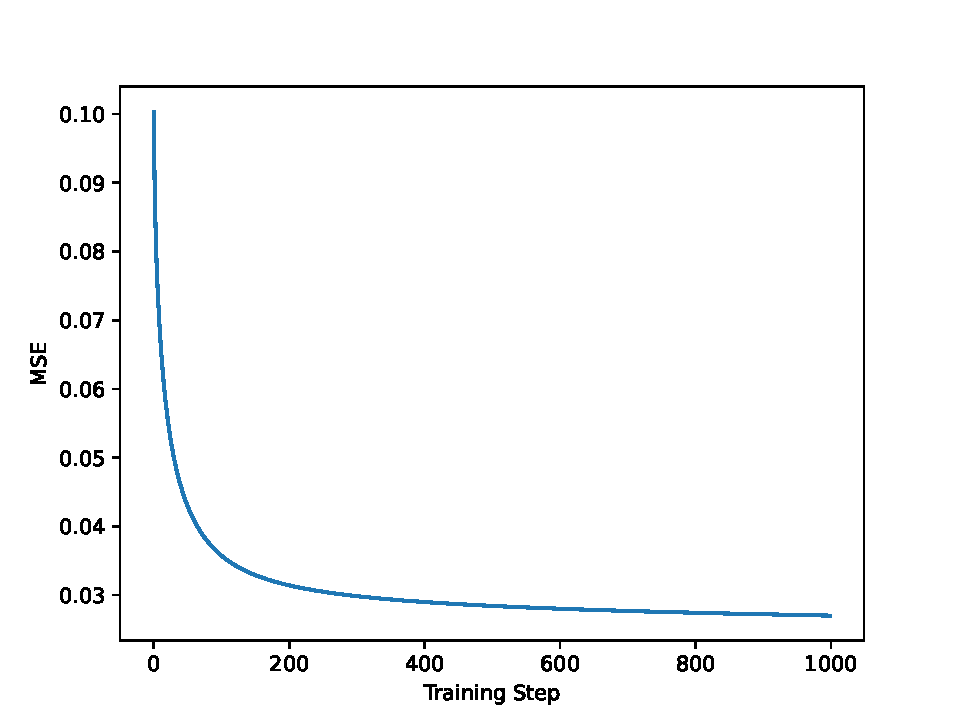
\includegraphics[width=0.6\linewidth]{imgs/MSE.pdf}
    \caption{MSE of the classifier during training}
    \label{fig:dist_mat}
\end{figure}
The MSE of the model quickly drops off at the start of the training and then starts to level off. After training the model for 1000 steps, the training set accuracy is 92.6\% and the test set accuracy is 86.5\%. Comparing these results to the accuracies of the distance-based models discussed before shows that the multiclass perceptron performs better than the naive distance-based approach. However, KNN outperforms the multiclass perceptron by $\sim5\%$ on both the training and test sets. 


\section{Task 3: XOR Network and Gradient Descent}
The structure we used in our neural network to solve the XOR problem is as followed. The pre-activation values $\mathbf{f}_0$ for the hidden layer are calculated from the input $\mathbf{x}$ by using the parameters $\boldsymbol{\Omega}$ and the bias $\boldsymbol{\beta}_0$. The hidden layer values $h_1,h_2$ are sequentially calculated using the sigmoid function. 
\begin{align*}
    \mathbf{f}_0 &= \boldsymbol{\beta}_0 + \boldsymbol{\Omega}\mathbf{x} \\    
    \mathbf{h} &= \sigma[\mathbf{f}_0]
\end{align*}
The output $\hat{y}$ is calculated similarly using the three parameters $\omega_1, \omega_2, \beta_1$. 
\begin{align*}
    f_1 &= \beta_1 + \omega_1h_1 + \omega_2h_2 = \beta_1 + \boldsymbol{\omega}^T\mathbf{h} \\
    \hat{y} &= \sigma[f_1]
\end{align*}
To train the network, we'll need to define a loss function $l$. The factor $\tfrac{1}{2}$ is to get rid of any constant factors in the backpropagation process.
\begin{align*}
    l &= \tfrac{1}{2}(\hat{y} - y)^2 = \tfrac{1}{2}(\sigma[f_1]-y)^2 
\end{align*}
We'll need the loss function's partial derivatives with respect to all (pre-)activation values to use backpropagation for the process of training the network using a gradient descent  algorithm.
\begin{align*}
    \tfrac{\partial l}{\partial f_1} &= (\sigma[f_1] - y)(1 - \sigma[f_1])\sigma[f_1] \\
    \tfrac{\partial f_1}{\partial \mathbf{h}} &= \boldsymbol{\omega} \\
    \tfrac{\partial \mathbf{h}}{\partial \mathbf{f}_0} &= \tfrac{\partial}{\partial \mathbf{f}_0} (\sigma[\mathbf{f}_0]) = \mathrm{diag}[\sigma[\mathbf{f}_0]\odot(1-\sigma[\mathbf{f}_0])] 
\end{align*}
While using the gradient descent algorithm, we're of course only interested in the gradients of the loss function with respect to the parameters, hence we need some more derivatives. We end up with a complete expression for every parameter.
\begin{align*}
    \tfrac{\partial l}{\partial \beta_1} &= \tfrac{\partial f_1}{\partial \beta_1} \tfrac{\partial l}{\partial f_1} = \tfrac{\partial l}{\partial f_1} \\
    \tfrac{\partial l}{\partial \boldsymbol{\omega}} &= \tfrac{\partial f_1}{\partial \boldsymbol{\omega}} \tfrac{\partial l}{\partial f_1} =  \tfrac{\partial l}{\partial f_1}\mathbf{h} \\
    \tfrac{\partial l}{\partial \boldsymbol{\beta}_0} &= \tfrac{\partial \mathbf{f}_0}{\partial \boldsymbol{\beta}_0} \tfrac{\partial \mathbf{h}}{\partial \mathbf{f}_0} \tfrac{\partial f_1}{\partial \mathbf{h}} \tfrac{\partial l}{\partial f_1}  = \mathbf{I} \tfrac{\partial \mathbf{h}}{\partial \mathbf{f}_0} \tfrac{\partial f_1}{\partial \mathbf{h}} \tfrac{\partial l}{\partial f_1}  \\
    \tfrac{\partial l}{\partial \boldsymbol{\Omega}} &=  \tfrac{\partial \mathbf{f}_0}{\partial \boldsymbol{\Omega}} \tfrac{\partial \mathbf{h}}{\partial \mathbf{f}_0} \tfrac{\partial f_1}{\partial \mathbf{h}} \tfrac{\partial l}{\partial f_1}  = \tfrac{\partial \mathbf{h}}{\partial \mathbf{f}_0} \tfrac{\partial f_1}{\partial \mathbf{h}} \tfrac{\partial l}{\partial f_1} \mathbf{x}^T
\end{align*}
While training the network, we recorded the mean squared error (MSE) to track its progress.
\begin{align*}
    \text{MSE} = \tfrac{1}{4}\Sigma_i^{4}(\hat{y}[\mathbf{x}_i] - y_i)^2
\end{align*}
After using the "lazy approach" to finding a decent combination of parameter initializations and learning rates, we initialized all parameters and biases using random values picked from a normal distribution centered around $0$ with a standard deviation of $0.5$. For our learning rate we used a value of $0.75$. 

We trained the model 100 times with ten thousand epochs, and we found that in 41\% of the networks, there were no classification errors. In 25\% there was a single error, and in the remaining 34\% of networks, there were two errors.

In figure \ref{fig:MSE_XOR} the MSE is plotted against the number of epochs during the training of three different neural networks. Two of the three networks make at least one classification error, hence their MSE is higher and only a local minimum is found during the gradient descent process. For the network with no errors, the MSE is visible a lot lower, almost zero, and a global minimum is found.

\begin{figure}
    \centering
    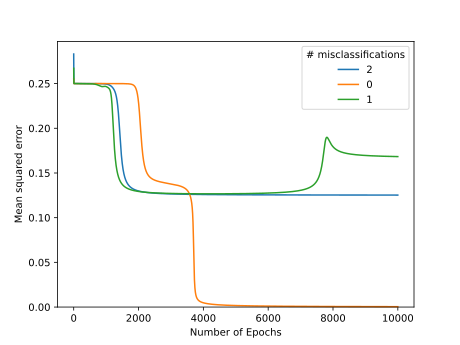
\includegraphics[width=0.5\linewidth]{TrainingExamplesXOR.svg}
    \caption{The MSE of three different XOR neural networks, one with 0, 1 and 2 classification errors.}
    \label{fig:MSE_XOR}
\end{figure}

\section{Contribution}
Phoebe: Task 1 code, Task 1 report\\
Vincent: Task 1 code, Task 3 code, Task 3 report\\
Niels: Task 1 code, Task 2 code, Task 2 report \\

\end{document}